\chapter{Massresolution}
Figure \ref{fig:massresolution_all} shows the fits to all bins of \Dz\proton mass for the determination of the massresolution.
The whole method and prodecure is described in section \ref{sec:Massresolution}.
\begin{figure}[hptb]
    \centering
	\includegraphics[width=0.32\textwidth]{LbToD0p/massresolution/massresolution_000}
	\includegraphics[width=0.32\textwidth]{LbToD0p/massresolution/massresolution_001}
	\includegraphics[width=0.32\textwidth]{LbToD0p/massresolution/massresolution_002} \\
	\includegraphics[width=0.32\textwidth]{LbToD0p/massresolution/massresolution_003}
	\includegraphics[width=0.32\textwidth]{LbToD0p/massresolution/massresolution_004}
	\includegraphics[width=0.32\textwidth]{LbToD0p/massresolution/massresolution_005} \\
	\includegraphics[width=0.32\textwidth]{LbToD0p/massresolution/massresolution_006}
	\includegraphics[width=0.32\textwidth]{LbToD0p/massresolution/massresolution_007}
	\includegraphics[width=0.32\textwidth]{LbToD0p/massresolution/massresolution_008} \\
	\includegraphics[width=0.32\textwidth]{LbToD0p/massresolution/massresolution_009}
	\includegraphics[width=0.32\textwidth]{LbToD0p/massresolution/massresolution_010}
	\includegraphics[width=0.32\textwidth]{LbToD0p/massresolution/massresolution_011} \\
	\includegraphics[width=0.32\textwidth]{LbToD0p/massresolution/massresolution_012}
	\includegraphics[width=0.32\textwidth]{LbToD0p/massresolution/massresolution_013}
	\includegraphics[width=0.32\textwidth]{LbToD0p/massresolution/massresolution_014} \\
	\includegraphics[width=0.32\textwidth]{LbToD0p/massresolution/massresolution_015}
	\includegraphics[width=0.32\textwidth]{LbToD0p/massresolution/massresolution_016}
	\includegraphics[width=0.32\textwidth]{LbToD0p/massresolution/massresolution_017} \\
	%\includegraphics[width=0.32\textwidth]{LbToD0p/massresolution/massresolution_018}
	%\includegraphics[width=0.32\textwidth]{LbToD0p/massresolution/massresolution_019}
	%\includegraphics[width=0.32\textwidth]{LbToD0p/massresolution/massresolution_020} \\
	%\includegraphics[width=0.32\textwidth]{LbToD0p/massresolution/massresolution_021}
	%\includegraphics[width=0.32\textwidth]{LbToD0p/massresolution/massresolution_022}
	%\includegraphics[width=0.32\textwidth]{LbToD0p/massresolution/massresolution_023} \\
	\caption{Fit of a Gaussian to the difference between generated and reconstructed \Dz\proton mass (simulation sample) in bins of 30\mev \Dz\proton) mass (first 18 bins of 24 shown here). The width of the Gaussian is taken as massresolution for the respective bin.}
    \label{fig:massresolution_all}
\end{figure}

\chapter{Reweighting of \LbToDpmunuX decay simulation}
\label{app:Reweight_D0p}
Figure \ref{fig:reweight_D0p_app} shows several more comparisons of data and simulation before and after reweighting.
More on the reweighting process can be found in section \ref{sec:Reweight_D0p}.
\begin{figure}[hptb]
    \centering
	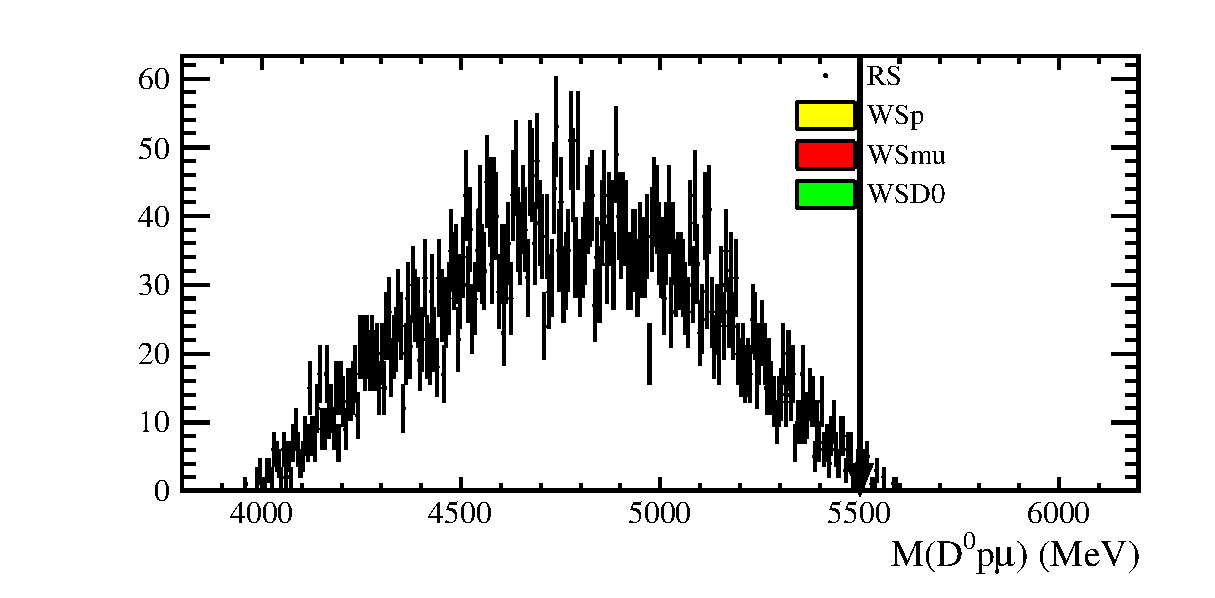
\includegraphics[width=0.32\textwidth]{LbToD0p/comparisons/3D/mD0p_mD0mu_mD0pmu/20Bins/20.0MaxWeight/Bh_M}
	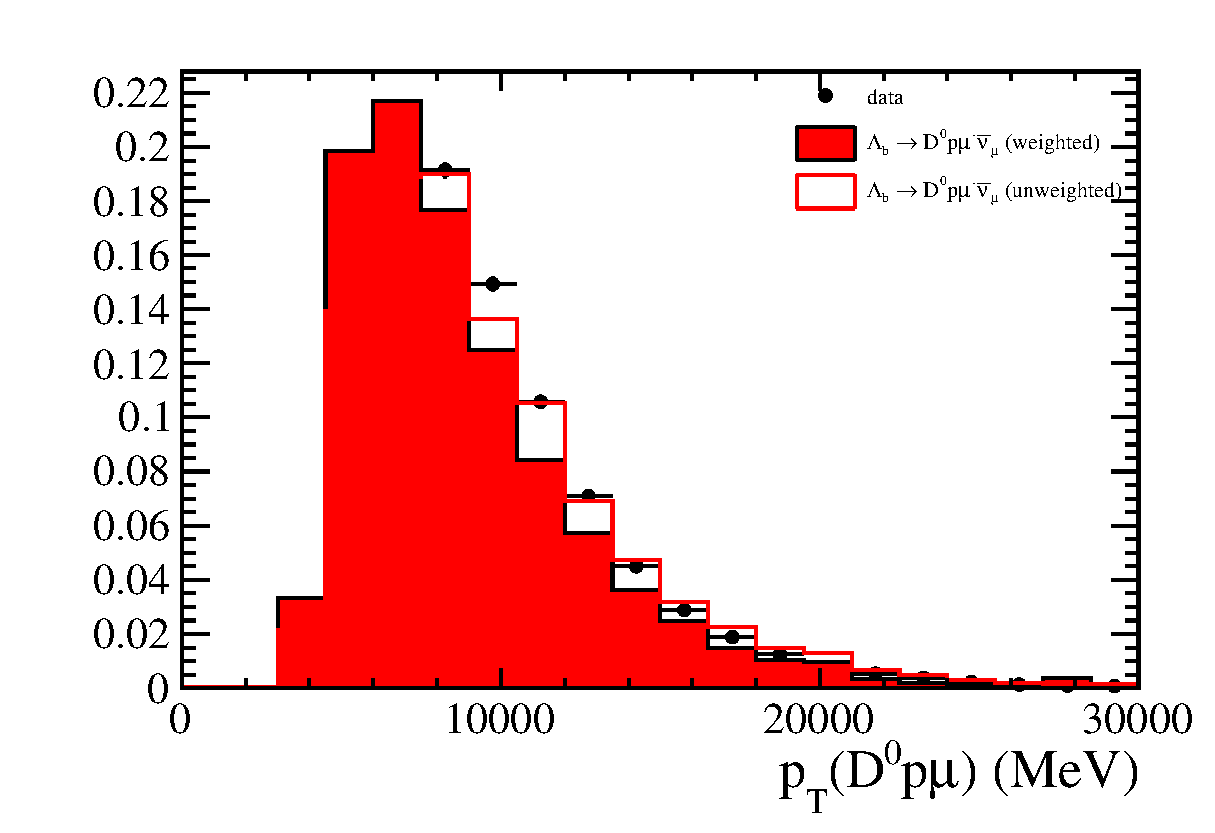
\includegraphics[width=0.32\textwidth]{LbToD0p/comparisons/3D/mD0p_mD0mu_mD0pmu/20Bins/20.0MaxWeight/Bh_PT}
	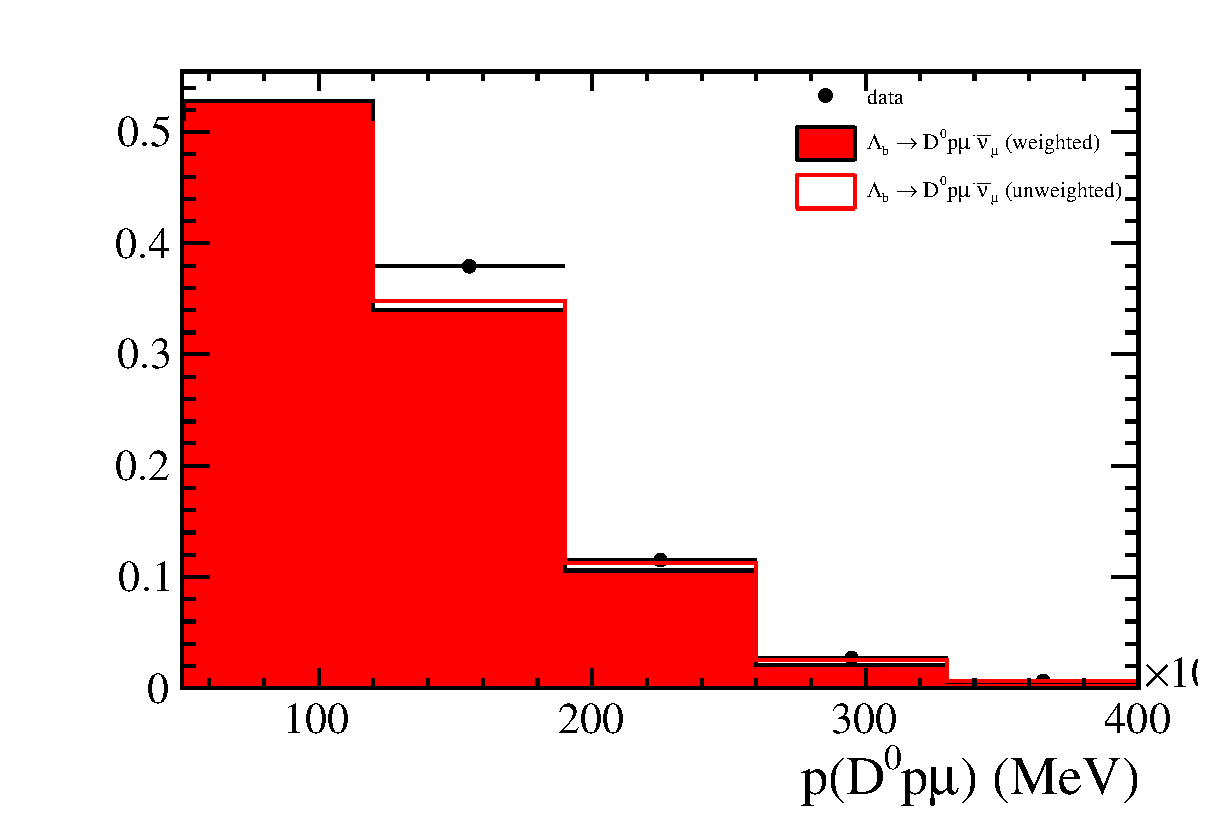
\includegraphics[width=0.32\textwidth]{LbToD0p/comparisons/3D/mD0p_mD0mu_mD0pmu/20Bins/20.0MaxWeight/Bh_P}          \\
	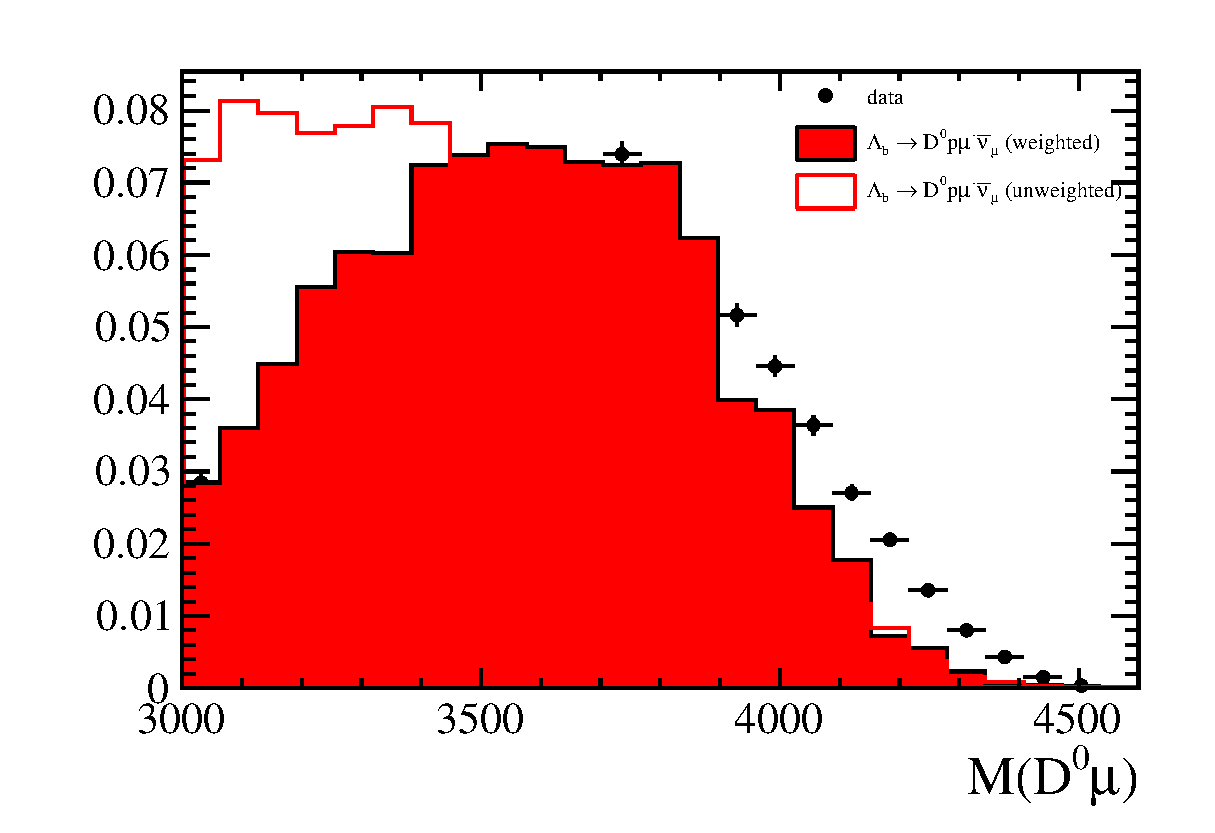
\includegraphics[width=0.32\textwidth]{LbToD0p/comparisons/3D/mD0p_mD0mu_mD0pmu/20Bins/20.0MaxWeight/B_M}           
	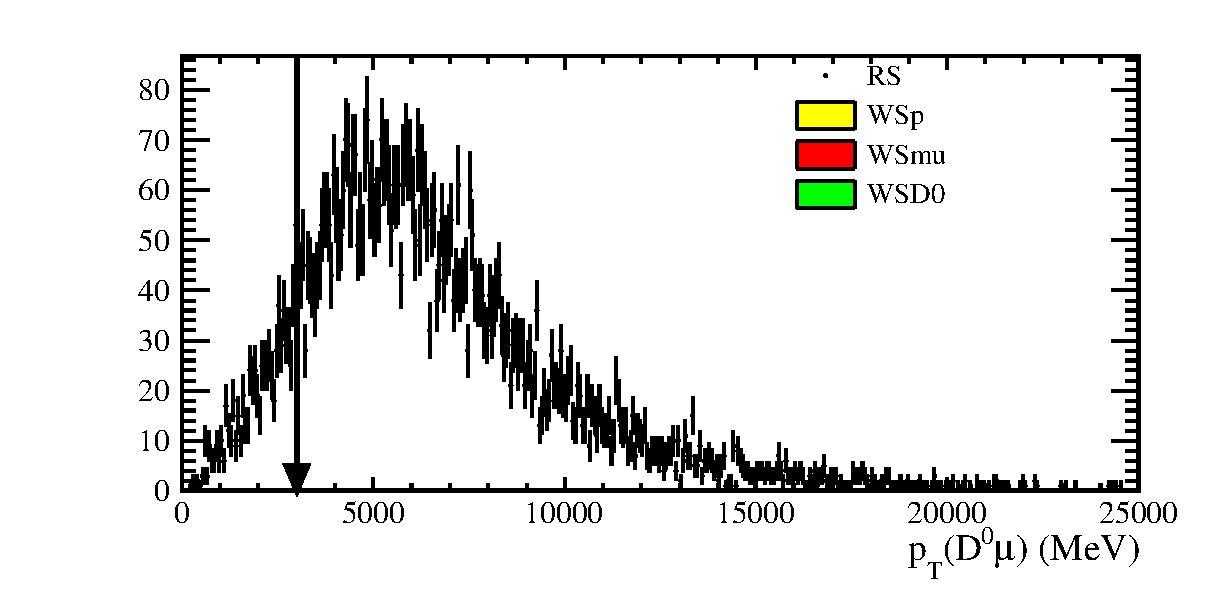
\includegraphics[width=0.32\textwidth]{LbToD0p/comparisons/3D/mD0p_mD0mu_mD0pmu/20Bins/20.0MaxWeight/B_PT}
	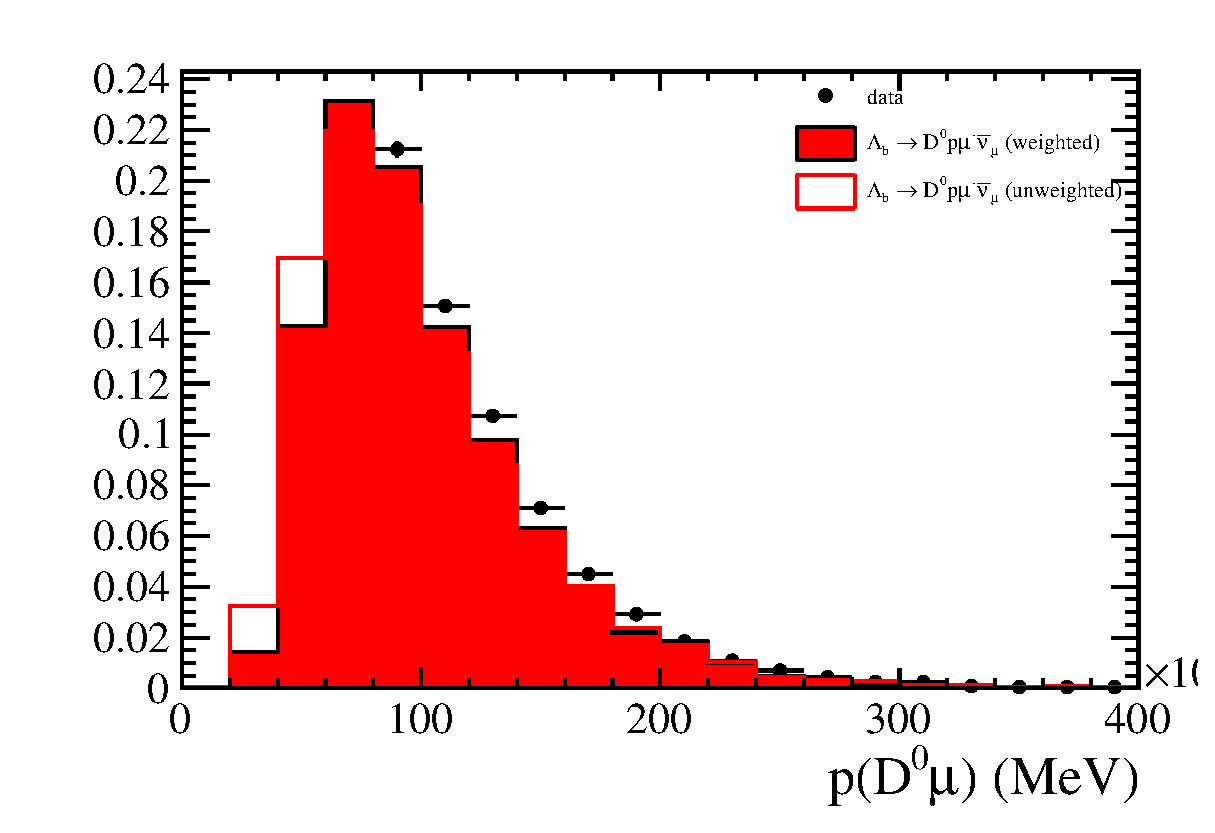
\includegraphics[width=0.32\textwidth]{LbToD0p/comparisons/3D/mD0p_mD0mu_mD0pmu/20Bins/20.0MaxWeight/B_P}           \\
    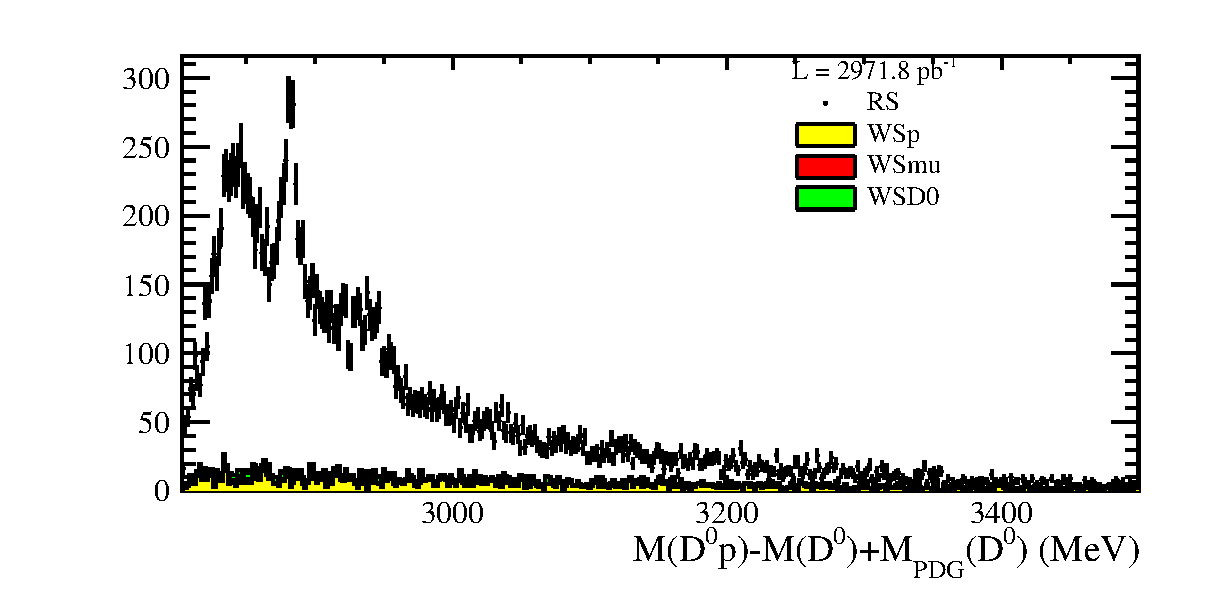
\includegraphics[width=0.32\textwidth]{LbToD0p/comparisons/3D/mD0p_mD0mu_mD0pmu/20Bins/20.0MaxWeight/Bh_DELTA_MASS}
	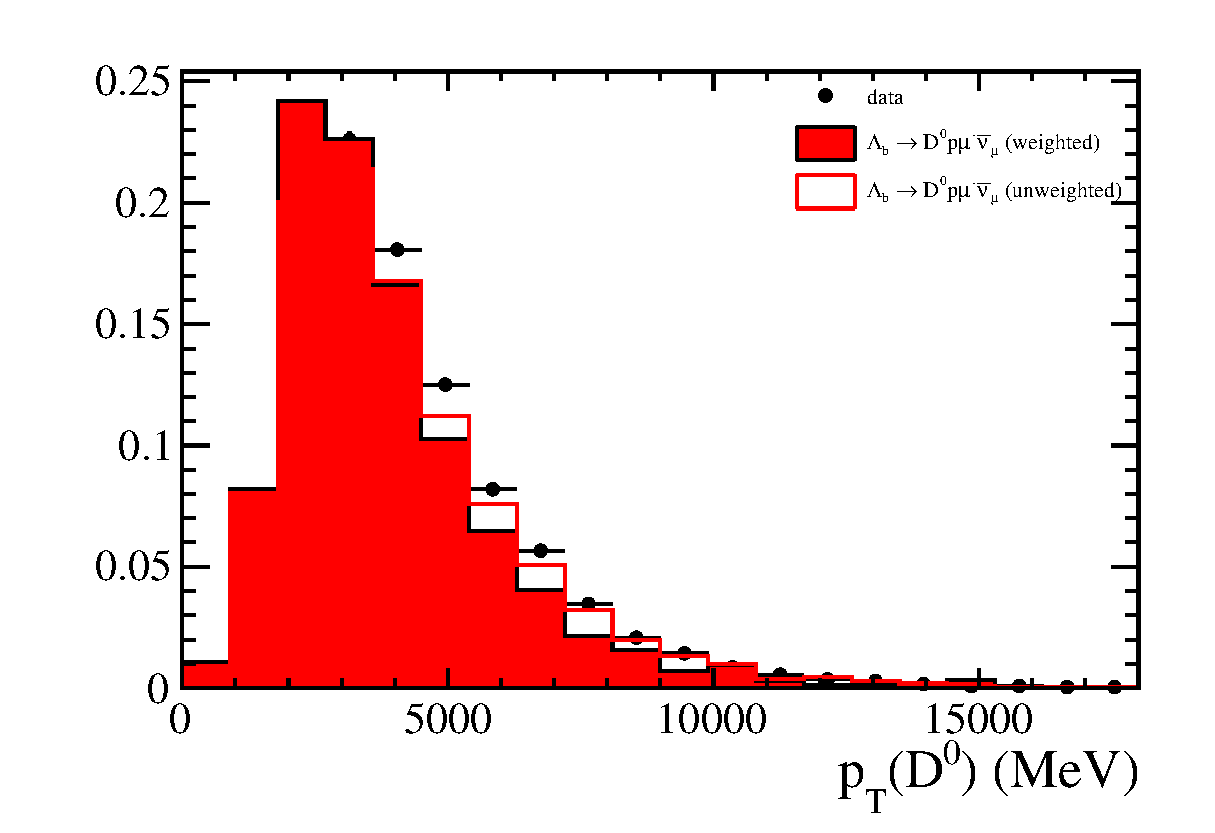
\includegraphics[width=0.32\textwidth]{LbToD0p/comparisons/3D/mD0p_mD0mu_mD0pmu/20Bins/20.0MaxWeight/D0_PT}
	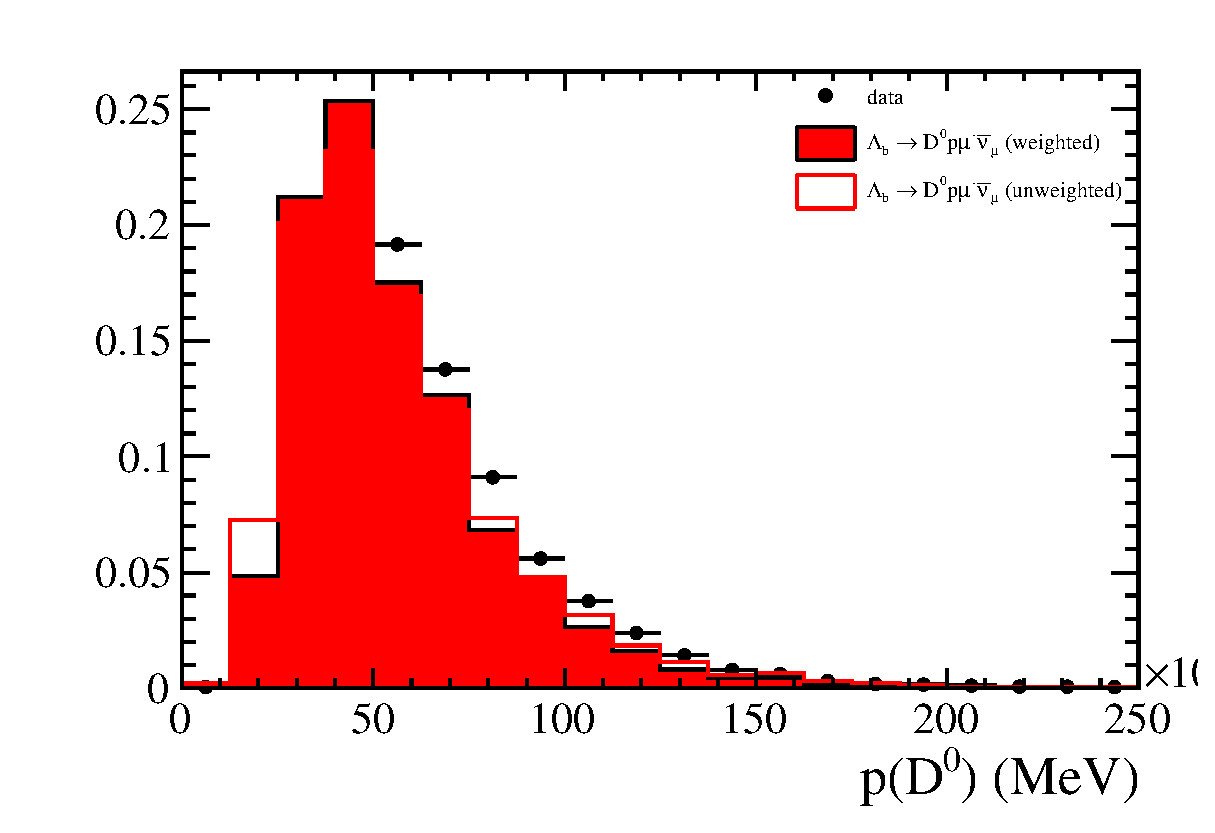
\includegraphics[width=0.32\textwidth]{LbToD0p/comparisons/3D/mD0p_mD0mu_mD0pmu/20Bins/20.0MaxWeight/D0_P}          \\
    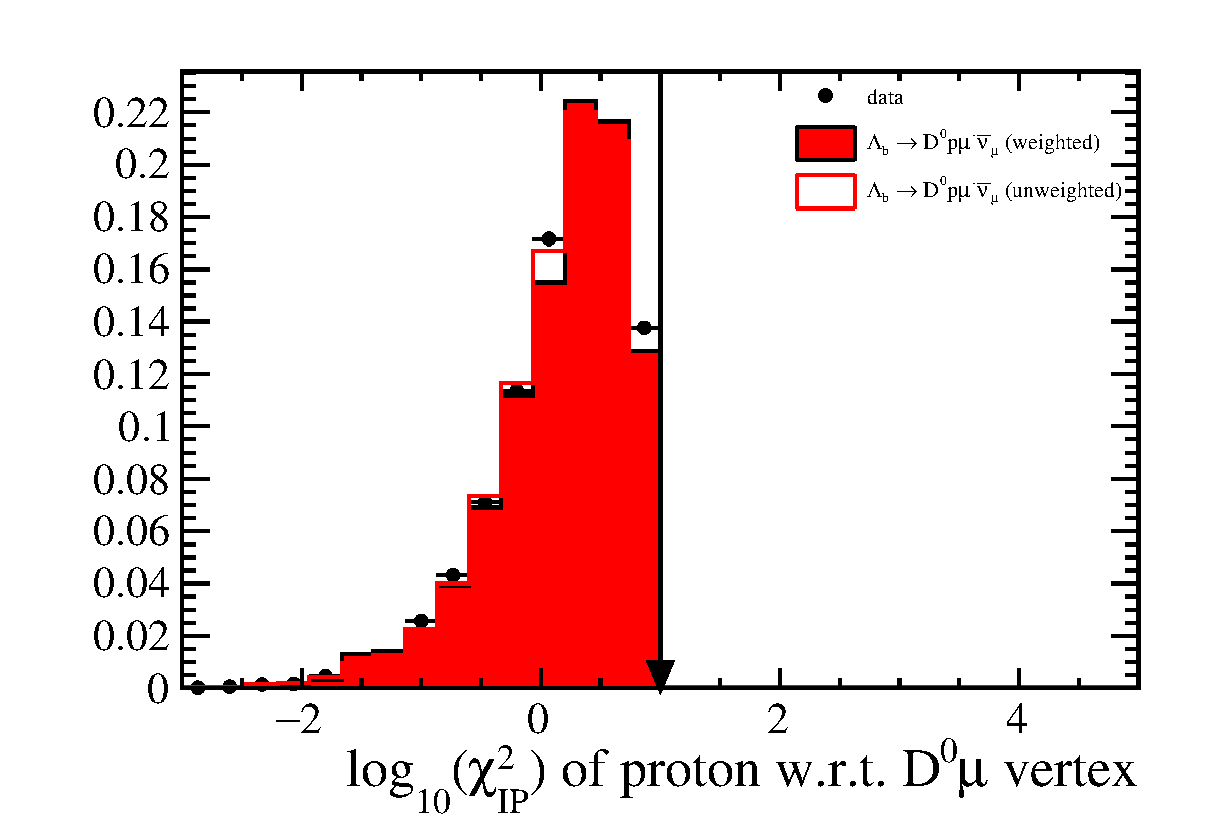
\includegraphics[width=0.32\textwidth]{LbToD0p/comparisons/3D/mD0p_mD0mu_mD0pmu/20Bins/20.0MaxWeight/logIP}
	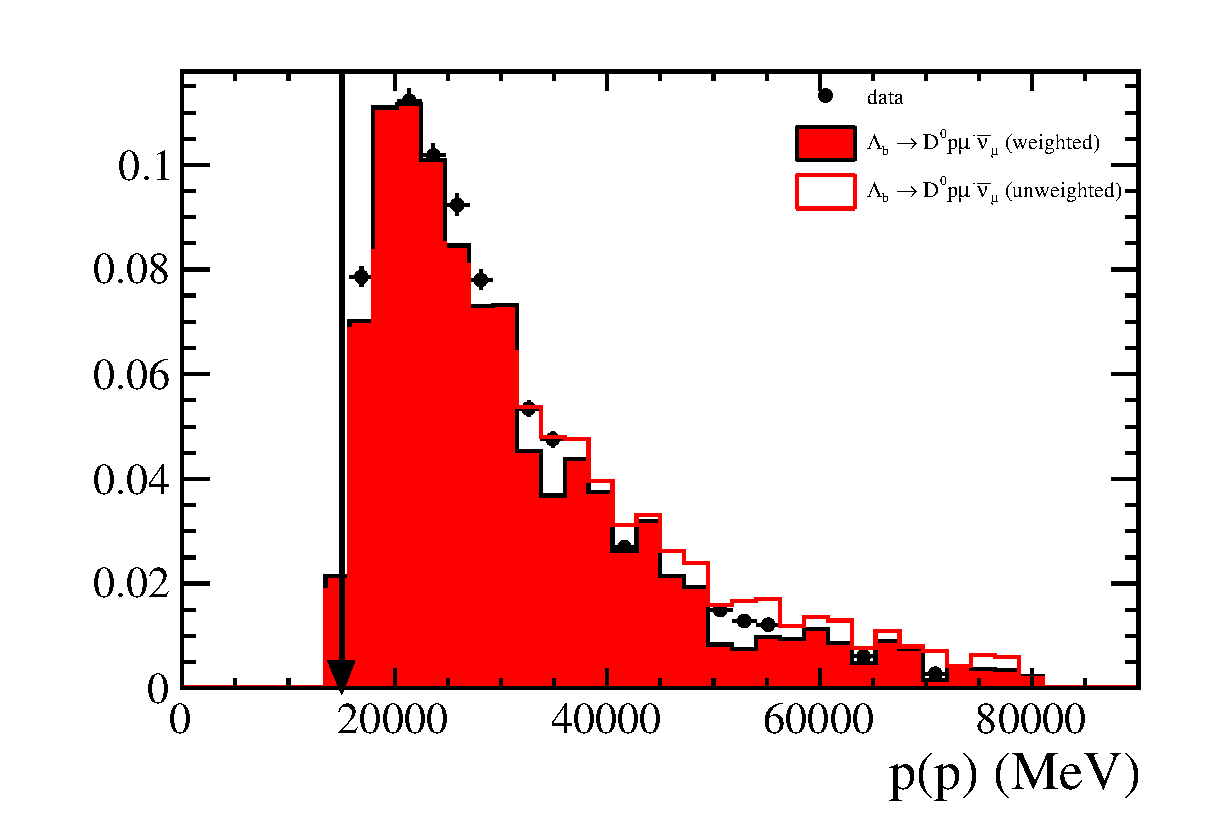
\includegraphics[width=0.32\textwidth]{LbToD0p/comparisons/3D/mD0p_mD0mu_mD0pmu/20Bins/20.0MaxWeight/h_P}
	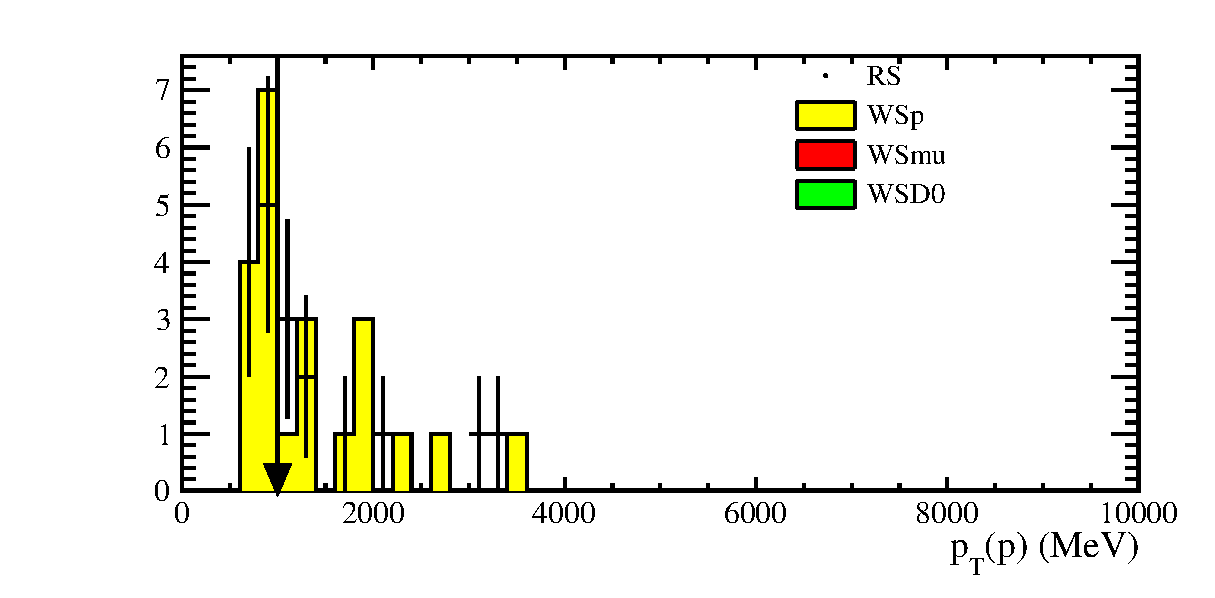
\includegraphics[width=0.32\textwidth]{LbToD0p/comparisons/3D/mD0p_mD0mu_mD0pmu/20Bins/20.0MaxWeight/h_PT}
	\caption{Comparison of data (black points) and simulation for the \LbToDpmunuX channel before (red line) and after (red shaded area) threedimensional reweighting as described in the text (see sec. \ref{sec:Reweight_D0p}).}
    \label{fig:reweight_D0p_app}
\end{figure}
